\documentclass[runningheads]{llncs}

\usepackage[T1]{fontenc}
\usepackage{amsmath,amssymb}
\usepackage{booktabs}
\usepackage{graphicx}
\usepackage{listings}
\usepackage{xcolor}
\usepackage{url}
\usepackage{array}

\newcommand{\tool}{\textsc{UpgradeGuard}}
\newcommand{\cmark}{\(\checkmark\)}
\newcommand{\pmark}{\(\triangle\)}
\newcommand{\xmark}{\(\times\)}
\newcommand{\sem}[1]{[\![#1]\!]}
\newcommand{\obs}{\mathsf{Obs}}
\newcommand{\dom}{\mathsf{Dom}}
\newcommand{\Safe}{\mathsf{Safe}}
\newcommand{\Unsafe}{\mathsf{Unsafe}}
\newcommand{\Unknown}{\mathsf{Unknown}}
\newcommand{\Timeout}{\mathsf{Timeout}}

\lstdefinelanguage{Solidity}{
  keywords={contract,function,external,returns,uint256,uint128,address,bool,
    mapping,require,emit,return,assembly,sstore,if,else,public,private,internal,
    payable,struct,unchecked},
  sensitive=true,
  morecomment=[l]{//},
  morecomment=[s]{/*}{*/},
  morestring=[b]"
}
\lstset{
  language=Solidity,
  basicstyle=\ttfamily\scriptsize,
  keywordstyle=\color{blue!55!black},
  commentstyle=\color{green!40!black},
  columns=fullflexible,
  keepspaces=true,
  frame=single,
  breaklines=true,
  showstringspaces=false
}

\begin{document}

\title{\tool: Compiler-Grounded Selective Relational Verification for Safe Solidity Upgrades}
\titlerunning{\tool: Selective Relational Verification for Solidity Upgrades}

\author{Bao Huynh \and Tuan-Dung Tran}
\authorrunning{B. Huynh and T.-D. Tran}
\institute{University of Information Technology, Vietnam National University, Ho Chi Minh City, Vietnam\\ \email{dungtrt@uit.edu.vn}}

\maketitle

\begin{abstract}
Proxy upgrades preserve an address and its storage while replacing the code that interprets them.  This creates two coupled hazards: a new implementation may reinterpret a persistent byte range, or a nominally preserved entry point may change its observable transition.  We present \tool, an offline analyzer that combines compiler-grounded storage footprints with selective relational verification.  A layout cell records slot, byte offset, width, semantic type, and path; a product obligation compares success status, return or revert data, events, external interactions, and related post-state.  Satisfiable obligations yield replayable counterexamples, unsatisfiable obligations certify the supported finite-domain model, and unsupported constructs remain explicit rather than being accepted optimistically.  We evaluate a deterministic corpus of 180 compiling Solidity upgrade pairs over 20 originals and 37 mutation operators, 43,200 measured analyzer executions, OpenZeppelin and bounded differential-fuzzing baselines, and Anvil replay.  On the controlled corpus, the storage analysis obtains precision 0.885 and recall 0.900; the behavioral analysis obtains precision 0.873 and recall 0.800.  Forty-eight solver counterexamples were independently reproduced on Anvil, whose Wilson 95\% lower bound is 0.926.  Median end-to-end time is 1.18--18.51\,ms across case classes.  The non-perfect results expose the present boundaries: identifier-only layout matching, computed assembly addresses, conditional effects, revert payloads, and cryptographic expressions.

\keywords{Upgradeable smart contracts \and Relational verification \and Storage layout \and SMT \and Solidity}
\end{abstract}

\section{Introduction}
\label{sec:introduction}

Upgradeable proxies decouple stable state from replaceable logic.  The pattern is operationally useful but weakens the usual intuition that deployed code is immutable: an administrator may redirect every subsequent delegate call while the proxy retains its old storage.  Recent empirical studies show both the prevalence and diversity of proxy mechanisms~\cite{li2024characterizing,zhang2025proxy}. EIP-1967 standardizes several administrative slots, but it does not constrain the implementation's ordinary state layout~\cite{eip1967}.  Consequently, an individually correct new version may still be an unsafe replacement.

Existing tools cover important parts of this problem.  OpenZeppelin compares compiler layouts~\cite{openzeppelin2025upgrades}; CRUSH detects storage collisions and CollisionRepair repairs them~\cite{ruaro2024crush,pan2025collisionrepair}. Recent single-version systems infer invariants, verify declarative contracts, or synthesize properties~\cite{chen2024invariants,chen2024dcv,liu2025propertygpt}; specialized analyzers target address checks and modified library guards~\cite{sun2024avverifier,liu2024zepscope}.  None of these ingredients alone states which old storage bytes a new version may reinterpret \emph{and} whether selected public transitions remain observationally equivalent.

We formulate replacement safety as a conjunction of physical layout compatibility and selective relational equivalence.  The word ``selective'' is essential: upgrades often intentionally add or change methods, so global bytecode equivalence is neither required nor desirable.  For each preserved method, \tool constructs a product formula and asks Z3~\cite{demoura2008z3} whether two related executions can be distinguished.  A model is checked by an independent concrete summary interpreter and replayed on a local EVM.

The contributions are a byte-accurate compatibility relation for packed cells, dynamic roots, inheritance, reserved gaps, and literal assembly writes; a selective product semantics over status, return or revert data, events, external interactions, and projected post-state; a four-valued verdict discipline that preserves \(\Unknown\) and \(\Timeout\) while producing replayable witnesses; and a controlled evaluation over 180 compiling upgrade pairs with repeated measurements, baselines, and component ablations.

The evaluation is deliberately controlled rather than presented as a real-world prevalence study.  Its imperfect outcomes identify the exact frontier of the implemented analysis and avoid converting unsupported syntax into apparent success.

\section{Background and Related Work}
\label{sec:related}

\subsection{Upgradeable storage}

Under \texttt{delegatecall}, implementation instructions read and write the proxy's storage.  Solidity assigns state variables according to inheritance, packing, and type-specific root rules~\cite{solidity2025layout}.  Mappings and dynamic arrays occupy a root slot whose descendants are hash-derived; moving the root therefore changes every logical cell even when the value type is unchanged.  Recent ecosystem studies characterize upgrade mechanisms and their security implications~\cite{li2024characterizing,zhang2025proxy}. CRUSH detects collisions and synthesizes exploits; CollisionRepair reconstructs slot ownership and patches affected systems~\cite{ruaro2024crush,pan2025collisionrepair}. Sorensen develops a mechanized upgrade framework in Coq~\cite{sorensen2024upgrades}.  Our focus is an executable two-version relation that joins layout preservation with selected behavioral obligations.

\subsection{Verification and testing}

Recent work illustrates three complementary directions.  DCV verifies declarative contracts by induction, invariant studies quantify which inferred properties are effective, and PropertyGPT retrieves and generates candidate specifications~\cite{chen2024dcv,chen2024invariants,liu2025propertygpt}. AVVerifier and ZepScope specialize program analysis to address validation and library-check consistency~\cite{sun2024avverifier,liu2024zepscope}, whereas CrySol combines replay and dynamic taint analysis for cryptographic defects~\cite{zhang2025crysol}.  Verification-service studies expose mismatches between published source and deployed bytecode~\cite{ma2024verification}; Osprey and iAudit respectively synthesize concrete attacks and justified audit findings~\cite{ruaro2025osprey,ma2025iaudit}.  Empirical evaluations nevertheless report substantial gaps between tool capabilities and practitioner needs~\cite{chaliasos2024tools,li2024sast}.  These systems analyze one version or one vulnerability family, while \tool asks whether two versions preserve a declared cross-version relation.

\begin{table*}[t]
\caption{Related-work capabilities in ascending publication year. \cmark~= support, \pmark~= partial support, and \xmark~= no support. Capability cells contain symbols only.}
\label{tab:related}
\centering
\scriptsize
\setlength{\tabcolsep}{3pt}
\resizebox{\textwidth}{!}{%
\begin{tabular}{lccccccc}
\toprule
Work & Year & Two-version & Layout & Behavior & CEx & EVM replay & Real corpus \\
\midrule
USCDetector~\cite{li2024characterizing} & 2024 & \pmark & \pmark & \xmark & \xmark & \xmark & \cmark \\
CRUSH~\cite{ruaro2024crush} & 2024 & \pmark & \cmark & \xmark & \cmark & \pmark & \cmark \\
Coq upgrades~\cite{sorensen2024upgrades} & 2024 & \cmark & \pmark & \pmark & \xmark & \xmark & \xmark \\
DCV~\cite{chen2024dcv} & 2024 & \xmark & \xmark & \pmark & \pmark & \xmark & \pmark \\
AVVerifier~\cite{sun2024avverifier} & 2024 & \xmark & \xmark & \pmark & \cmark & \pmark & \cmark \\
ZepScope~\cite{liu2024zepscope} & 2024 & \xmark & \xmark & \pmark & \cmark & \pmark & \cmark \\
Verification services~\cite{ma2024verification} & 2024 & \pmark & \xmark & \xmark & \cmark & \pmark & \cmark \\
ProxyEx~\cite{zhang2025proxy} & 2025 & \pmark & \pmark & \xmark & \xmark & \cmark & \cmark \\
PropertyGPT~\cite{liu2025propertygpt} & 2025 & \xmark & \xmark & \pmark & \pmark & \xmark & \cmark \\
CrySol~\cite{zhang2025crysol} & 2025 & \xmark & \xmark & \pmark & \cmark & \cmark & \cmark \\
CollisionRepair~\cite{pan2025collisionrepair} & 2025 & \pmark & \cmark & \xmark & \cmark & \pmark & \cmark \\
Osprey~\cite{ruaro2025osprey} & 2025 & \xmark & \xmark & \pmark & \cmark & \cmark & \cmark \\
\tool{} (this work) & 2026 & \cmark & \pmark & \pmark & \cmark & \cmark & \xmark \\
\bottomrule
\end{tabular}
}
\end{table*}

Table~\ref{tab:related} intentionally does not give \tool full coverage. Computed assembly addressing is unresolved, behavioral verification covers a documented Solidity subset, and the evaluation corpus is controlled rather than mined from production histories.

\section{Relational Upgrade-Safety Model}
\label{sec:problem}

Let \(V_i=(C_i,\mathcal L_i)\) denote implementation code and compiler storage layout for version \(i\in\{1,2\}\).  A layout entry for variable \(v\) is
\begin{equation}
\lambda_i(v)=\bigl(s_i(v),o_i(v),w_i(v),\tau_i(v),\pi_i(v)\bigr),
\label{eq:cell}
\end{equation}
where \(s\) is a 32-byte slot, \(o\) a byte offset, \(w\) a byte width, \(\tau\) a semantic type, and \(\pi\) the declaration path induced by inheritance.  Its physical footprint is
\begin{equation}
B_i(v)=\{32s_i(v)+o_i(v),\ldots,
32s_i(v)+o_i(v)+w_i(v)-1\}.
\label{eq:footprint}
\end{equation}
For a mapping or dynamic array, \(B_i(v)\) denotes the root; the derived addressing function remains part of \(\tau_i(v)\).

To distinguish physical coincidence from semantic compatibility, define the byte-interpretation map \(\mu_i:\mathbb{N}\rightarrow\mathcal{T}\times\mathcal{P}\times\mathbb{N}\) by
\begin{equation}
\mu_i(b)=\bigl(\tau_i(v),\pi_i(v),b-\min B_i(v)\bigr)\quad\text{for the unique }v\text{ such that }b\in B_i(v).
\label{eq:byte-interpretation}
\end{equation}
For a mapping key \(k\) and a dynamic-array index \(j\), descendant locations are generated by
\begin{equation}
\alpha_i^{\mathrm{map}}(v,k)=H(\operatorname{enc}(k)\Vert\operatorname{enc}(s_i(v))),\qquad
\alpha_i^{\mathrm{arr}}(v,j)=H(\operatorname{enc}(s_i(v)))+\left\lfloor\frac{jw_i(v)}{32}\right\rfloor .
\label{eq:root-addressing}
\end{equation}
Hence equality of root slots alone is insufficient: the recursive type must induce the same descendant-address language.

Let \(P_1\) be the old variables whose values must persist.  A partial correspondence \(\rho:P_1\rightharpoonup P_2\) is compatible when
\begin{equation}
\forall v\in P_1:\quad
B_1(v)=B_2(\rho(v))\ \land\
\tau_1(v)\simeq\tau_2(\rho(v)),
\label{eq:layout-compatible}
\end{equation}
and \(\rho\) is injective.  Equivalently, compatibility requires \(\mu_1(b)=\mu_2(b)\) for every persistent byte after paths are transported by \(\rho\).  The relation \(\simeq\) requires equal recursive encoding for roots and equal signedness and width for scalar interpretation. New variables are allowed only outside \(\bigcup_{v\in P_1}B_1(v)\), except that a suffix of a declared gap may be consumed without moving its retained suffix.

For public method \(f\), we model one execution as
\begin{equation}
\sem{f}_{i}(\sigma,a,\kappa)
  =(q_i,r_i,d_i,e_i,x_i,\sigma'_i),
\label{eq:transition}
\end{equation}
where \(\sigma\) is storage, \(a\) arguments and sender context, \(\kappa\) the modeled external-call result, \(q\) success status, \(r\) return bytes, \(d\) revert bytes, \(e\) the ordered event trace, and \(x\) the ordered external-call trace.  The observable projection is
\begin{equation}
\obs_\rho(t_i)=
\bigl(q_i,\ q_i?r_i:d_i,\ e_i,\ x_i,\
      \sigma'_i\!\downarrow_{\dom(\rho)}\bigr).
\label{eq:observation}
\end{equation}
Including failure payloads and interaction order prevents a weak post-state-only notion of equivalence.

For each preserved method, the distinguishability set collects all related executions with unequal observations:
\begin{equation}
\Delta_f(\rho)=\left\{(\sigma_1,\sigma_2,a,\kappa)\ \middle|\;
\sigma_1\sim_\rho\sigma_2,\ (a,\kappa)\in D_f,\;
\obs_\rho(\sem{f}_1(\sigma_1,a,\kappa))\neq\obs_\rho(\sem{f}_2(\sigma_2,a,\kappa))
\right\}.
\label{eq:distinguishability-set}
\end{equation}

\begin{definition}[Selective upgrade safety]
Given preserved methods \(M_p\) and input domains \(D_f\), the upgrade \(V_1\leadsto V_2\) is safe relative to \((\rho,M_p,D)\) iff
\begin{equation}
\mathsf{Compat}_{\mathcal{L}}(\rho)\ \land\
\bigcup_{f\in M_p}\Delta_f(\rho)=\varnothing ,
\label{eq:selective-safety}
\end{equation}
where \(\mathsf{Compat}_{\mathcal{L}}\) abbreviates Eq.~\eqref{eq:layout-compatible}, injectivity, descendant-address preservation, and non-overlap with newly allocated cells.
\end{definition}

\section{Compiler-Grounded Relational Verification}
\label{sec:design}

\begin{figure}[t]
\centering
\fbox{\parbox[c][38mm][c]{0.94\linewidth}{
\centering
\textbf{Architecture placeholder}\\[2mm]
\texttt{solc artifacts}
\(\longrightarrow\) layout relation and assembly scan\\
\(\longrightarrow\) function mapper and product encoder\\
\(\longrightarrow\) Z3 verdict and model\\
\(\longrightarrow\) concrete interpreter and Anvil replay\\[2mm]
\emph{Replace this box with the final external architecture artwork.}
}}
\caption{\tool architecture placeholder.  The final overview drawing will be inserted as an external vector asset.}
\label{fig:architecture}
\end{figure}

Figure~\ref{fig:architecture} summarizes the four stages.  The implementation consumes ABI, AST, bytecode, and \texttt{storageLayout} artifacts emitted in a single pinned \texttt{solc} invocation.

\subsection{Compiler-grounded layout relation}

The implemented full configuration first instantiates correspondence by the compiler-emitted declaration label, then checks physical position and normalized recursive type.  This deliberately conservative identity rule can reject an internal rename, a limitation isolated by the ID and S+T ablations.  For an old cell \(v\) and candidate \(u\), the compatibility predicate is
\begin{equation}
\begin{split}
K(v,u)={}&[s_1(v)=s_2(u)]\land[o_1(v)=o_2(u)]\\
&{}\land[w_1(v)=w_2(u)]\land[\tau_1(v)\simeq\tau_2(u)].
\end{split}
\label{eq:cell-compatibility}
\end{equation}
Let \(\nu_i(v)\) be the compiler label.  The prototype uses the partial map \(\rho_N(v)=u\) iff \(\nu_1(v)=\nu_2(u)\), and emits a component-wise diagnostic rather than collapsing every failure into one Boolean:
\begin{equation}
\boldsymbol{\ell}(v,u)=
\bigl(
[s_1(v)\neq s_2(u)],\,
[o_1(v)\neq o_2(u)],\,
[w_1(v)\neq w_2(u)],\,
[\tau_1(v)\not\simeq\tau_2(u)]
\bigr),
\qquad
\mathsf{Compat}_{\mathcal L}(\rho_N)\Longleftrightarrow
\sum_{v\in P_1}\|\boldsymbol{\ell}(v,\rho_N(v))\|_1=0.
\label{eq:layout-diagnostic}
\end{equation}
Missing labels are deletion diagnostics.  The checker additionally validates gap shrinkage and scans Yul/assembly for literal \texttt{sstore} destinations that overlap compiler-managed cells.  A computed destination is conservatively \(\Unknown\), because syntactic constant folding would be incomplete.

\subsection{Selective relational obligation}

Unchanged methods are skipped after canonical comparison.  For each changed preserved method, the frontend extracts guards, writes, returns, events, calls, and effect order.  Two summaries share symbolic pre-state and arguments.  The counterexample formula is
\begin{equation}
\begin{split}
\Phi_f={}&I_\rho(\sigma_1,\sigma_2)\land D_f(a,\kappa)\\
&{}\land T_{1,f}(\sigma_1,a,\kappa,t_1)
\land T_{2,f}(\sigma_2,a,\kappa,t_2)\\
&{}\land\neg\bigl(\obs_\rho(t_1)=\obs_\rho(t_2)\bigr).
\end{split}
\label{eq:product}
\end{equation}
If \(\Phi_f\) is satisfiable, its model is a regression witness.  If unsatisfiable, equivalence holds for the encoded semantics and declared domain.  Unsupported expressions produce \(\Unknown\); solver resource exhaustion produces \(\Timeout\).

The final lattice prioritizes evidence:
\begin{equation}
\Unsafe\succ\Timeout\succ\Unknown\succ\Safe.
\label{eq:verdict}
\end{equation}
Thus a definite layout collision is not hidden by an unrelated unsupported method, and an unsupported operation is never silently certified.

\subsection{Counterexample checking}

A solver model \(m\) is accepted only if a separately implemented concrete summary evaluator reproduces the observation difference.  The artifact then deploys both compiled versions on Anvil, initializes equal logical state using \texttt{anvil\_setStorageAt}, invokes the changed method, and compares call status/data, receipt status, logs, storage, and filtered opcode traces.  Replay uses batches of four fresh chains to bound provider state and isolate failures.

\begin{figure}[t]
\centering
\begin{minipage}[t]{0.47\linewidth}
\begin{lstlisting}[caption={Old version.},captionpos=b]
struct Account {
 uint128 credit;
 uint64 nonce;
 bool frozen;
}
mapping(address => Account) accounts;
uint128 total;
address payable treasury;

function withdraw(uint128 amount,
 uint64 expected) external {
  Account storage a = accounts[msg.sender];
  require(!a.frozen &&
          a.nonce == expected, "auth");
  require(a.credit >= amount, "balance");
  a.credit -= amount;
  a.nonce += 1;
  total -= amount;
  emit Withdrawn(msg.sender, amount,
                 a.nonce);
  (bool ok,) =
    msg.sender.call{value: amount}("");
  require(ok, "transfer");
}
\end{lstlisting}
\end{minipage}\hfill
\begin{minipage}[t]{0.47\linewidth}
\begin{lstlisting}[caption={Candidate version.},captionpos=b]
// [L1] moved before legacy cells
address payable treasury;
struct Account {
 // [L2] widened/repacked
 uint256 credit;
 bool frozen;
 uint64 nonce;
}
// [L3] mapping root shifted
mapping(address => Account) accounts;
uint128 total;

function withdraw(uint128 amount,
 uint64 expected) external {
  Account storage a = accounts[msg.sender];
  // [B1] replayable nonce accepted
  require(!a.frozen &&
          a.nonce <= expected, "auth");
  // [B2] recipient and order changed
  (bool ok,) =
    treasury.call{value: amount}("");
  require(ok, "transfer");
  // [B3] balance guard removed
  unchecked { a.credit -= amount; }
  total -= amount;
  // [B4] payload/stale nonce
  emit Withdrawn(msg.sender, total,
                 a.nonce);
}
\end{lstlisting}
\end{minipage}
\caption{A compound unsafe upgrade.  L1--L3 shift the mapping root and alter recursive value encoding; B1--B4 weaken authorization and balance guards, move and redirect the external interaction, suppress the nonce transition, and alter the event payload.}
\label{fig:example}
\end{figure}

Figure~\ref{fig:example} illustrates why upgrade safety cannot be reduced to either layout equality or equal post-state on common successful inputs.  Let \(s_i\) be the compiler-reported root of \texttt{accounts}.  For address \(x\) and field offset \(\delta_i\), the persistent cell is \(\alpha_i(x)=H(\operatorname{enc}(x)\Vert\operatorname{enc}(s_i))+\delta_i\); L1--L3 imply \((s_1,\delta_1,\tau_1)\neq(s_2,\delta_2,\tau_2)\).  Independently, choose the relational pre-state
\begin{equation}
a.\mathit{credit}=\mathit{amount}>0,\quad \mathit{total}\geq\mathit{amount},\quad a.\mathit{nonce}=n=\mathit{expected},\quad \neg a.\mathit{frozen},\quad \mathit{treasury}\neq\mathit{msg.sender}.
\label{eq:listing-witness}
\end{equation}
The old transition pays \(\mathit{msg.sender}\), increments the nonce to \(n+1\), and emits \((\mathit{amount},n+1)\); the candidate pays \(\mathit{treasury}\), leaves the nonce at \(n\), and emits \((\mathit{total}-\mathit{amount},n)\).  Thus Eq.~\eqref{eq:listing-witness} instantiates \(\Delta_{\mathrm{withdraw}}(\rho)\), while the root mismatch independently falsifies \(\mathsf{Compat}_{\mathcal L}(\rho)\).  The example therefore demonstrates both conjuncts of Eq.~\eqref{eq:selective-safety}, not merely a syntactic diff.

\subsection{Conditional guarantee and complexity}

\begin{theorem}
\label{thm:trace}
Assume Eq.~\eqref{eq:layout-compatible}, exact transition encodings \(T_{i,f}\), and \(\Phi_f\) unsatisfiable for every \(f\in M_p\).  Any finite client trace containing only calls in \(M_p\), with contexts in \(D_f\), has equal observations under \(V_1\) and \(V_2\).
\end{theorem}

\begin{proof}
By induction on trace length.  Initially the stores satisfy \(I_\rho\). For the inductive step, unsatisfiability of Eq.~\eqref{eq:product} excludes an observable difference for the next call and establishes related projected post-state.  This post-state is the induction hypothesis for the remaining trace.  The result follows for every finite length.
\end{proof}

The assumptions are explicit: the implementation's behavioral frontend is not an exact semantics for arbitrary Solidity.  For \(n\) layout cells, \(d\) changed preserved functions, and formula construction sizes \(g_f\), layout indexing costs \(O(n\log n)\), frontend work costs \(O(\sum_{f=1}^{d}g_f)\), and SMT solving remains theory-dependent.  Skipping unchanged methods makes \(d\), rather than the total public-method count, the dominant number of obligations.

\section{Experimental Evaluation}
\label{sec:evaluation}

\subsection{Dataset and experimental configuration}

The evaluation asks four questions: \textbf{RQ1} measures storage-regression detection against compiler-grounded mutations and OpenZeppelin; \textbf{RQ2} measures behavioral regression detection against a 128-trial deterministic differential baseline; \textbf{RQ3} isolates the accuracy, coverage, and latency contributions of analyzer components; and \textbf{RQ4} measures scaling with the number and symbolic-path mass of relational obligations.

We generate 20 originals spanning ten contract families and alternating transparent/UUPS metadata.  Each original has 7--8 functions and eight storage variables, including inheritance, packed scalars, a mapping, and either a dynamic array or gap.  Three independently generated upgrades per category give the balanced disjoint union
\begin{equation}
\mathcal{D}=\mathcal{D}_{\mathrm{safe}}\mathbin{\dot\cup}
\mathcal{D}_{\mathrm{layout}}\mathbin{\dot\cup}
\mathcal{D}_{\mathrm{behavior}},\qquad
|\mathcal{D}_{\mathrm{safe}}|
=|\mathcal{D}_{\mathrm{layout}}|
=|\mathcal{D}_{\mathrm{behavior}}|=60.
\label{eq:dataset-partition}
\end{equation}
Table~\ref{tab:dataset} reports the complete balance.

\begin{table}[t]
\caption{Controlled corpus composition.  ``S-unsafe'' and ``B-unsafe'' denote storage and behavioral regressions.}
\label{tab:dataset}
\centering
\scriptsize
\begin{tabular}{@{}
>{\raggedright\arraybackslash}m{0.34\columnwidth}
>{\raggedright\arraybackslash}m{0.58\columnwidth}@{}}
\toprule
Property & Corpus configuration \\
\midrule
Original contracts & 20 contracts from 10 application families \\
Application families & Access control, crowdfunding, escrow, marketplace, registry, reward distribution, staking, token, vault, and voting \\
Proxy patterns & 10 Transparent and 10 UUPS instances \\
Upgrade pairs & 180 independently generated V1--V2 pairs \\
Ground-truth balance & 60 safe, 60 S-unsafe, and 60 B-unsafe pairs \\
Mutation vocabulary & 37 safe, layout, behavioral, and unsupported operators \\
Contract structure & 7--8 public or external functions and eight compiler-visible storage variables per original \\
Solidity version & All V1 and V2 sources compile with Solidity 0.8.30 \\
\bottomrule
\end{tabular}
\end{table}

The 37 operators include compatible appends, gap consumption, alpha-renaming, equivalent arithmetic, reordered independent writes, declaration insertion, packing/type changes, mapping and array root motion, inheritance changes, literal and computed assembly writes, guard/arithmetic mutations, omitted or conditional writes/events, access-control removal, external-recipient/order changes, revert-data changes, and unsupported hash returns.  Every pair compiles with Solidity 0.8.30.  Ground truth is validated independently from the proposed detector by checking mutation realization in source and compiler artifacts; it is not defined by whether \tool succeeds.  Unlike recent large-scale vulnerability-corpus construction~\cite{chen2026forge}, this construction prioritizes controlled cross-version contrasts over incident coverage.  It separates three effects that mined corpora usually confound: proxy pattern, mutation semantics, and implementation family.  Consequently, a detector is evaluated on the intended cross-version relation rather than on vulnerability labels inherited from a different single-version task.

\textbf{Protocol and metrics.} OpenZeppelin Upgrades Core is run on all safe/storage cases.  The behavioral baseline executes 128 deterministic differential trials per safe/behavior case.  We count \(\Unknown\) and \(\Timeout\) on unsafe cases as false negatives, rather than deleting them.  Precision, recall, and \(F_1\) have their standard confusion-matrix definitions.  Boundary estimates are printed as Wilson one-sided limits instead of unjustified exact zeros or ones.

After three warmups, the full pipeline and seven ablations are each measured 30 times: 5,400 full and 37,800 ablation records.  RQ4 adds 300 batch observations.  All raw per-run rows are retained.  Experiments ran on Windows 11, an AMD Ryzen 7 7840HS (8 cores/16 threads), and 32\,GB RAM, with Python 3.12.10, Z3 4.13.4, Node 22.13.0, and Anvil 1.7.1.  Source code, seeds, raw measurements, and replication artifacts will be made available upon acceptance.

\begin{figure*}[t]
\centering
\begin{minipage}[t]{0.238\textwidth}
\centering
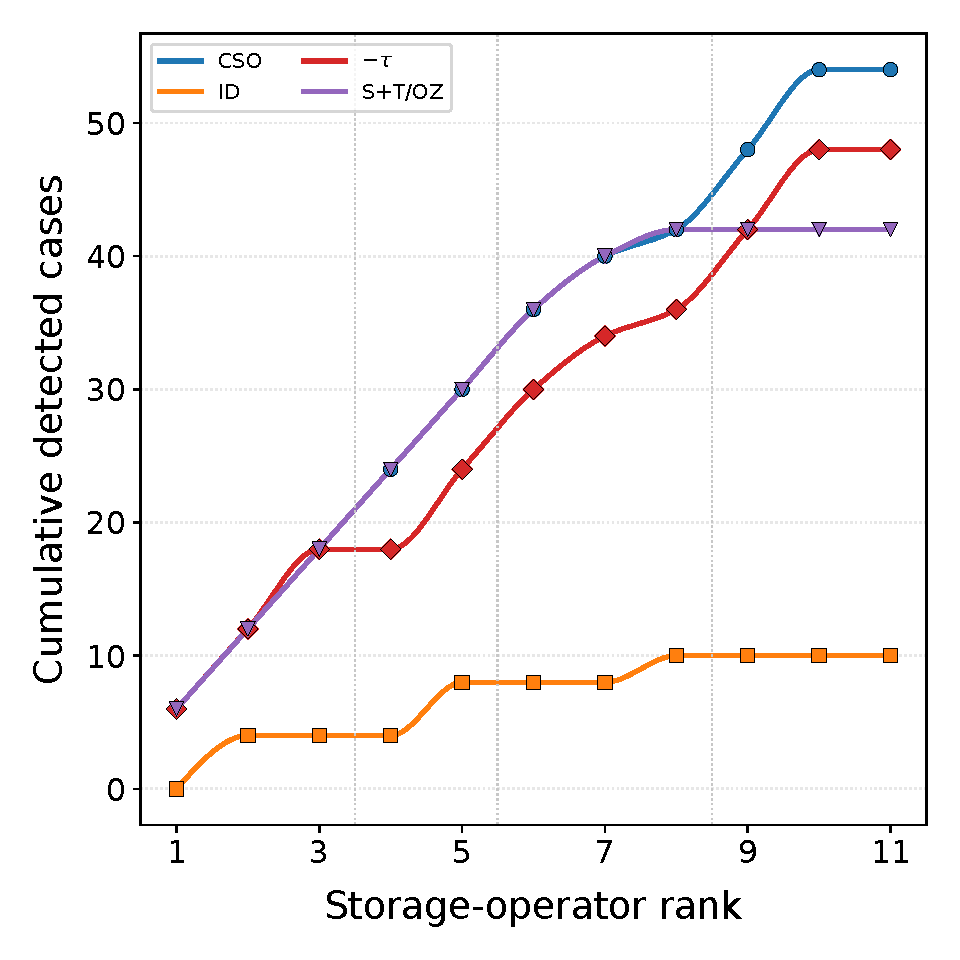
\includegraphics[width=\linewidth]{dataset/results/figures/figure_storage_1a_profile.pdf}\\[-1mm]
\scriptsize (a) Storage detection
\end{minipage}\hfill
\begin{minipage}[t]{0.238\textwidth}
\centering
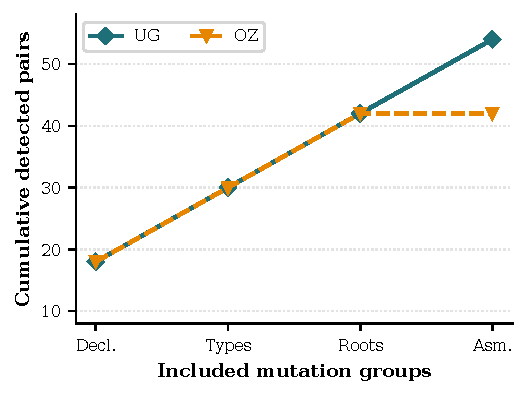
\includegraphics[width=\linewidth]{dataset/results/figures/figure_storage_1b_cumulative.pdf}\\[-1mm]
\scriptsize (b) Ablation profile
\end{minipage}\hfill
\begin{minipage}[t]{0.238\textwidth}
\centering
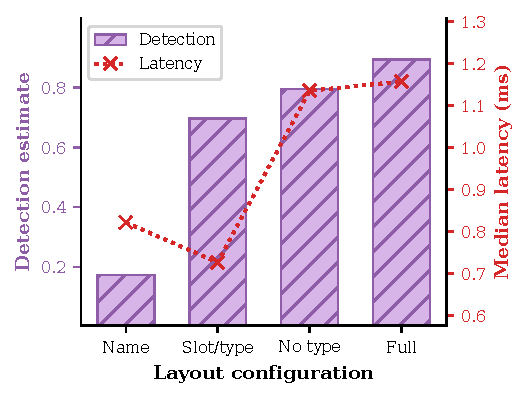
\includegraphics[width=\linewidth]{dataset/results/figures/figure_storage_1c_sensitivity.pdf}\\[-1mm]
\scriptsize (c) Layout latency
\end{minipage}\hfill
\begin{minipage}[t]{0.238\textwidth}
\centering
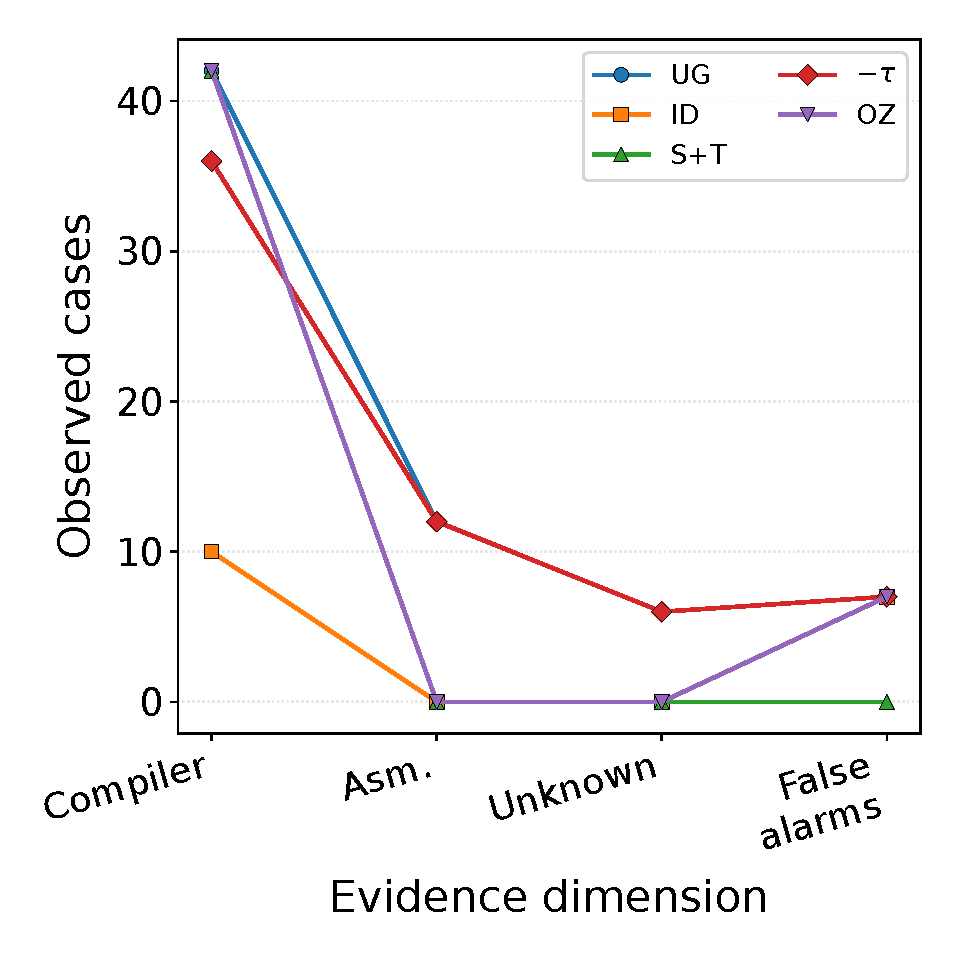
\includegraphics[width=\linewidth]{dataset/results/figures/figure_storage_1d_operators.pdf}\\[-1mm]
\scriptsize (d) Storage evidence
\end{minipage}

\smallskip
\begin{minipage}[t]{0.238\textwidth}
\centering
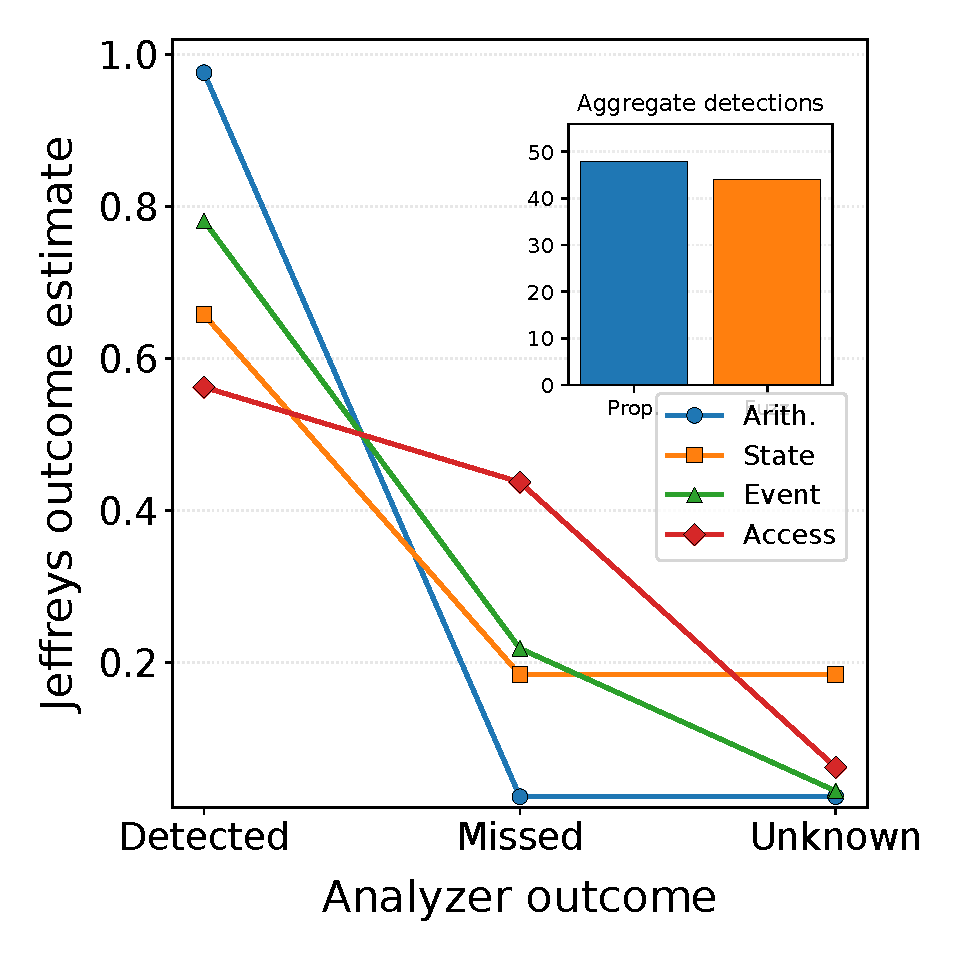
\includegraphics[width=\linewidth]{dataset/results/figures/figure_behavior_2a_profile.pdf}\\[-1mm]
\scriptsize (e) Outcome profile
\end{minipage}\hfill
\begin{minipage}[t]{0.238\textwidth}
\centering
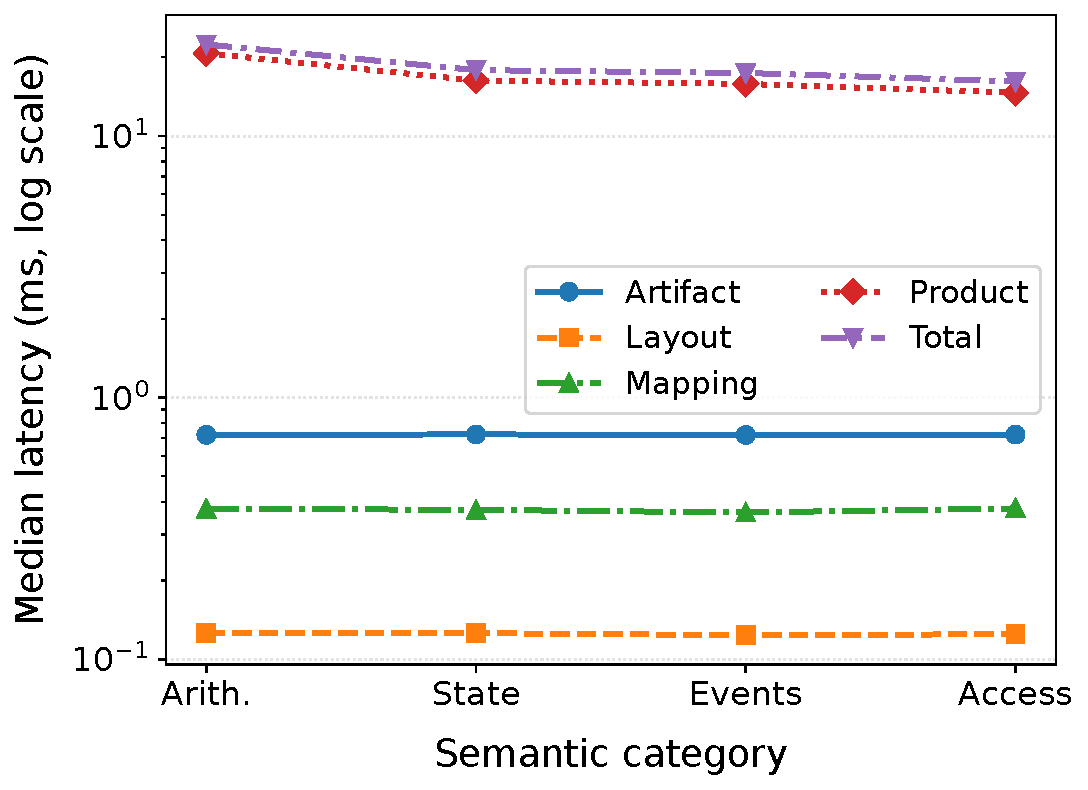
\includegraphics[width=\linewidth]{dataset/results/figures/figure_behavior_2b_latency.pdf}\\[-1mm]
\scriptsize (f) Verification density
\end{minipage}\hfill
\begin{minipage}[t]{0.238\textwidth}
\centering
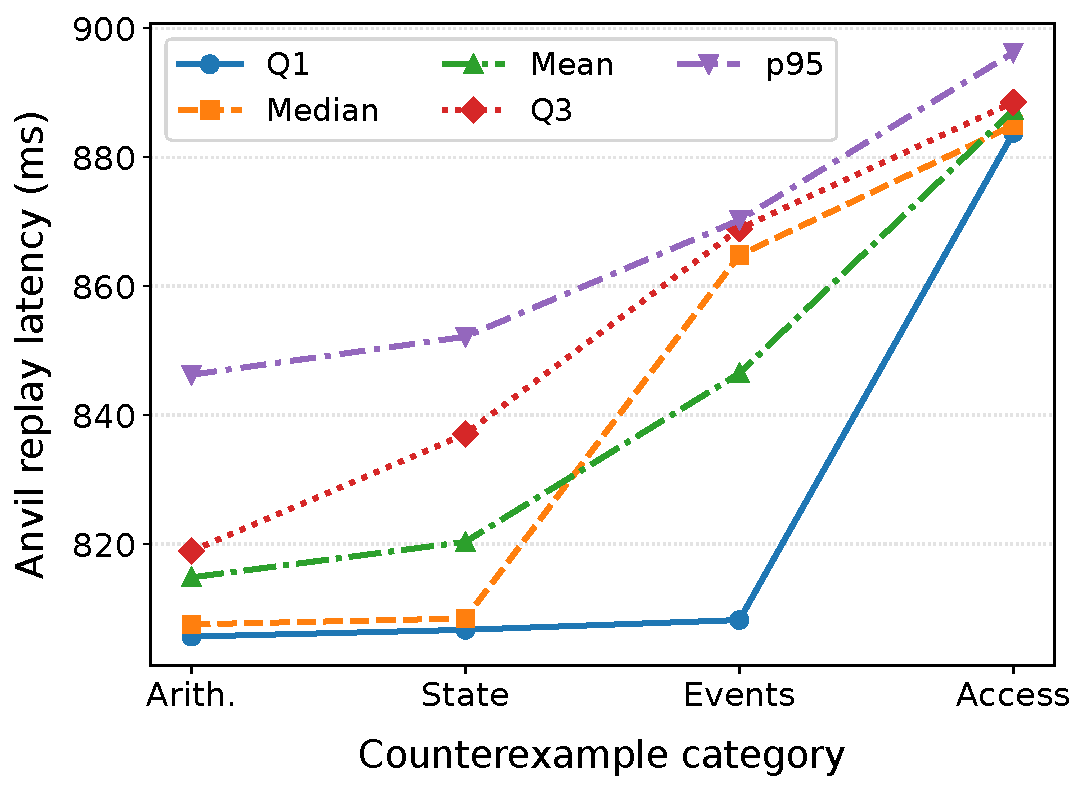
\includegraphics[width=\linewidth]{dataset/results/figures/figure_behavior_2c_replay.pdf}\\[-1mm]
\scriptsize (g) Replay quantiles
\end{minipage}\hfill
\begin{minipage}[t]{0.238\textwidth}
\centering
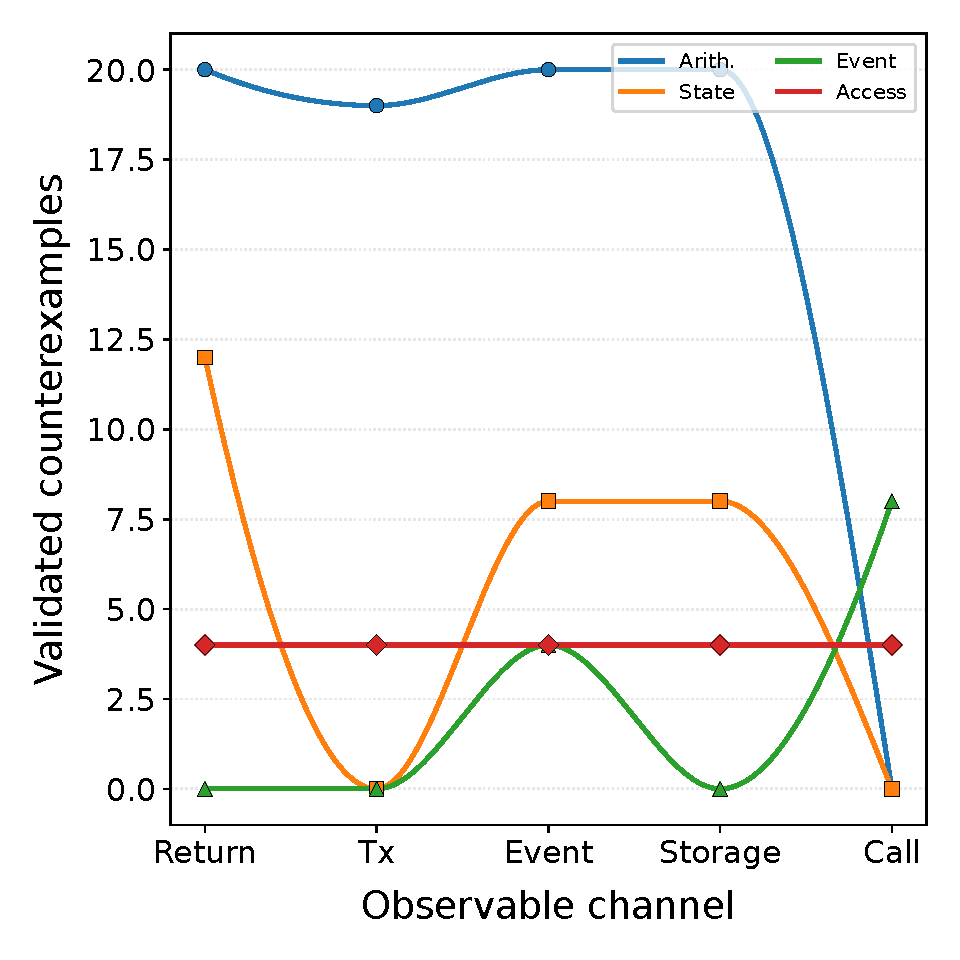
\includegraphics[width=\linewidth]{dataset/results/figures/figure_behavior_2d_observables.pdf}\\[-1mm]
\scriptsize (h) Evidence profiles
\end{minipage}
\caption{Detection and validation results.  The first row reports (a) posterior storage-family detection, (b) five-configuration ablation across classification criteria, (c) layout-latency density, and (d) storage evidence.  The second row reports (e) behavioral outcomes, (f) verification density, (g) replay quantiles, and (h) posterior EVM-evidence support. Legends abbreviate the proposed method as UG, identifier matching as ID, slot--offset--type matching as S+T, removal of type checking as \(-\tau\), and OpenZeppelin as OZ.  S+T and OZ coincide in panel (a).}
\label{fig:effectiveness}
\end{figure*}

\subsection{RQ1: storage compatibility}

\tool detects 54 of the 60 storage regressions, yielding precision 0.885, recall 0.900, and \(F_1=0.893\); OpenZeppelin reaches recall 0.700.  The smooth posterior profiles in Fig.~\ref{fig:effectiveness}(a) expose where each matcher loses mutation-family evidence.  Identifier matching loses root-moving mutations, removal of \(\tau\) loses equal-width type changes, and S+T cannot recover assembly destinations absent from the compiler layout.  The six unresolved cases compute an \texttt{sstore} destination and are conservatively classified as \(\Unknown\).

Panel (c) estimates the log-time density without changing observations:
\begin{equation}
 u_{m,i}=\log T_{m,i},\qquad
 \widehat f_m(u)=\frac{1}{n_mh_m}\sum_{i=1}^{n_m}
 K\!\left(\frac{u-u_{m,i}}{h_m}\right),
\label{eq:kde}
\end{equation}
where \(m\) indexes the analyzer configuration, \(K\) is a Gaussian kernel, and \(h_m\) follows Scott's rule.  The separated modes show that simplified matchers are faster because they discard evidence, not because they optimize the complete compatibility relation.

\subsection{RQ2: behavioral equivalence}

The relational checker reports 48 counterexamples, nine false proofs, and three \(\Unknown\) outcomes over the 60 behavioral regressions.  Its recall 0.800 exceeds the deterministic differential baseline's 0.733.  Arithmetic mutations account for the four additional detections in Fig.~\ref{fig:effectiveness}(e); conditional state, event, and revert-payload mutations account for the nine false proofs, while three hash-based returns remain explicitly unsupported.

All 48 SMT witnesses were reproduced on Anvil, with Wilson lower bound 0.926 and median replay latency 808.98\,ms.  Panel (h) summarizes each witness by the binary evidence vector
\begin{equation}
 \boldsymbol{\omega}
 =(\omega_{\mathrm{return}},\omega_{\mathrm{tx}},
   \omega_{\mathrm{event}},\omega_{\mathrm{store}},
   \omega_{\mathrm{call}})\in\{0,1\}^{5}.
\label{eq:evidence-vector}
\end{equation}
For class \(c\) and channel \(j\), panel (h) reports the Jeffreys posterior mean
\begin{equation}
 \widehat p_{c,j}=\frac{n_{c,j}+\tfrac12}{n_c+1},
\label{eq:evidence-support}
\end{equation}
where \(n_{c,j}\) counts validated witnesses exhibiting channel \(j\). Its five curves distinguish storage evidence from counterexamples corroborated by status, events, and external-interaction traces; shape-preserving interpolation is used only between the marked estimates.

\subsection{RQ3: ablation and performance}

\begin{figure*}[t]
\centering
\begin{minipage}[t]{0.322\textwidth}
\centering
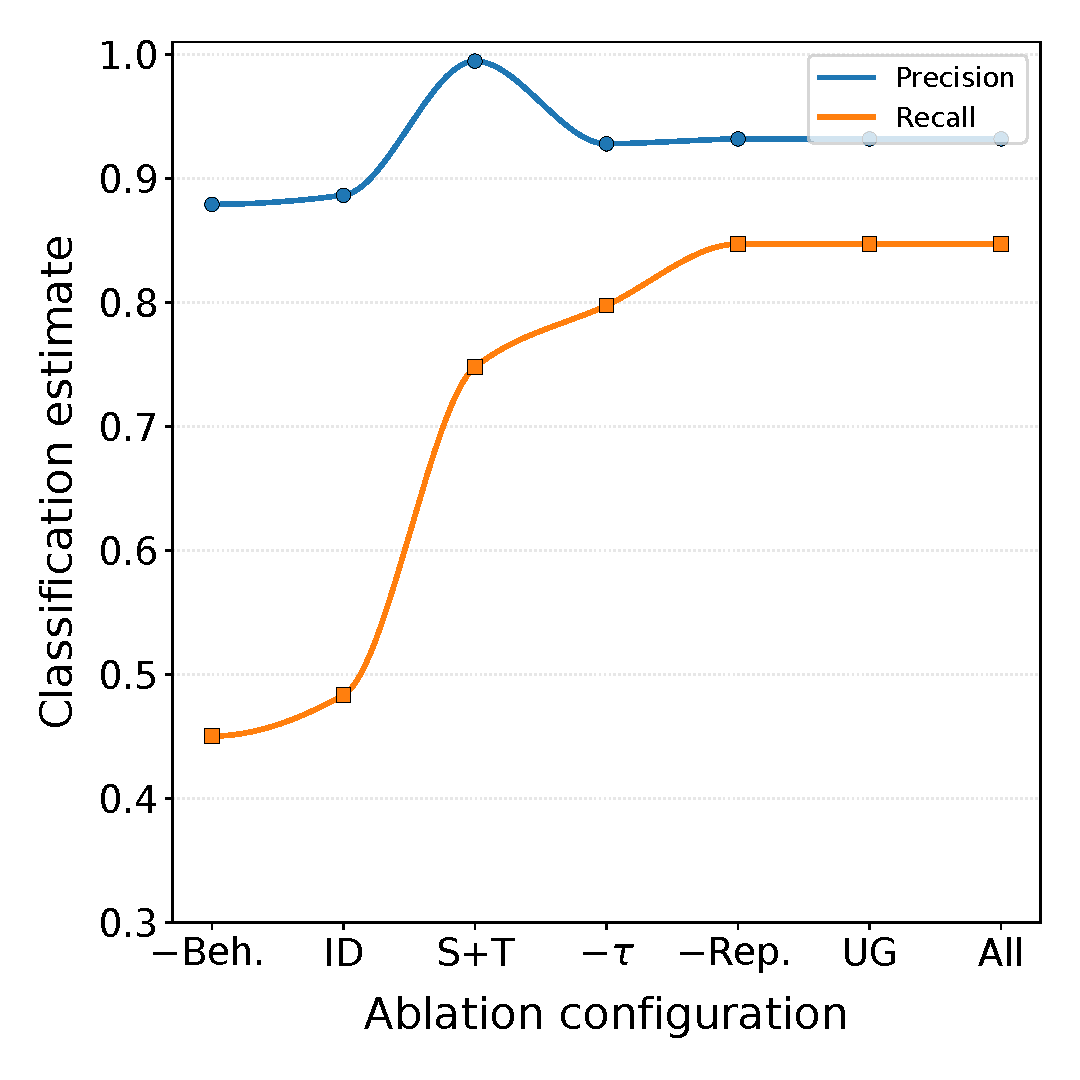
\includegraphics[width=\linewidth]{dataset/results/figures/figure_diagnostics_3a_quality.pdf}\\[-1mm]
\scriptsize (a) Precision and recall
\end{minipage}\hfill
\begin{minipage}[t]{0.322\textwidth}
\centering
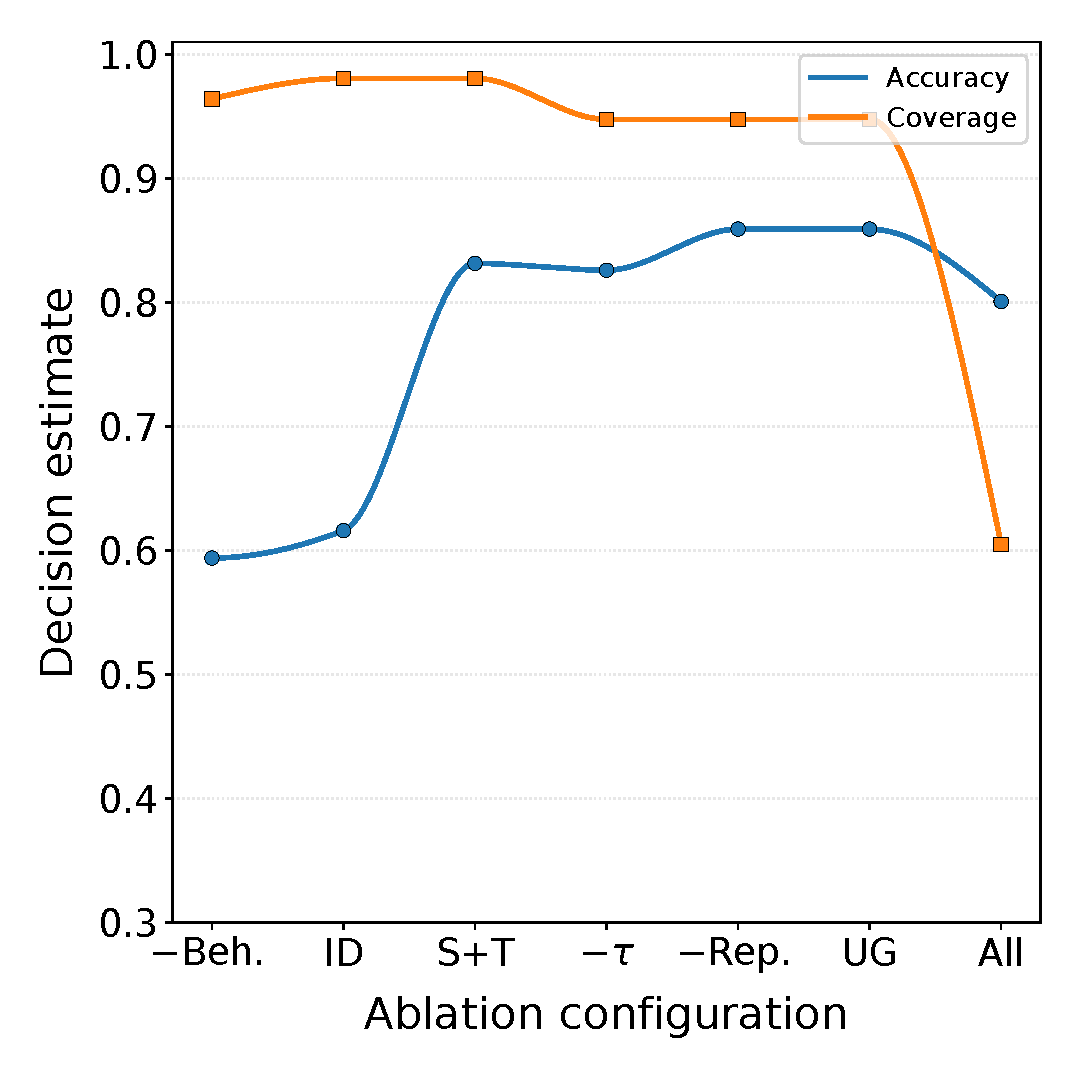
\includegraphics[width=\linewidth]{dataset/results/figures/figure_diagnostics_3b_decision.pdf}\\[-1mm]
\scriptsize (b) Accuracy and coverage
\end{minipage}\hfill
\begin{minipage}[t]{0.322\textwidth}
\centering
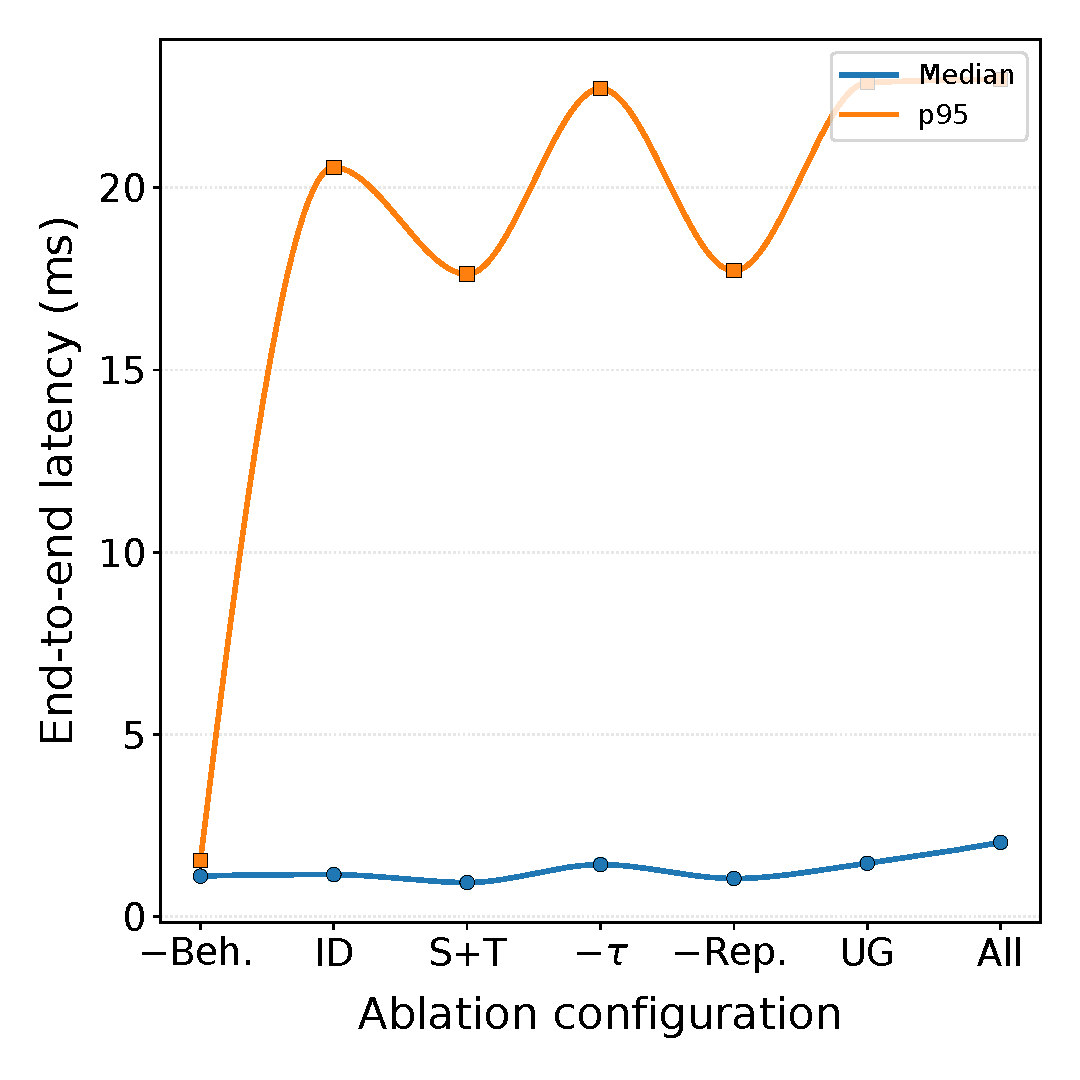
\includegraphics[width=\linewidth]{dataset/results/figures/figure_diagnostics_3c_runtime.pdf}\\[-1mm]
\scriptsize (c) Median and tail latency
\end{minipage}
\caption{Component ablation with a shared configuration order and plotting grammar.  Panel (a) separates precision from recall, panel (b) separates correctness from the fraction receiving a definite verdict, and panel (c) contrasts median with p95 end-to-end latency.  Curves connect Jeffreys estimates or measured timing summaries; no experimental value is altered.}
\label{fig:diagnostics}
\end{figure*}

The full configuration has Jeffreys accuracy 0.859, precision 0.932, recall 0.847, and decision coverage 0.948.  Removing behavioral reasoning lowers recall to 0.450, while identifier-only layout matching reaches 0.483; Fig.~\ref{fig:diagnostics}(a) shows that the loss is primarily sensitivity rather than precision.  Slot--offset--type matching has high precision 0.995 but recall 0.748 because it cannot recover assembly evidence.  Figure~\ref{fig:diagnostics}(b) exposes a different failure: analyzing all functions preserves precision and recall on decided cases but lowers coverage to 0.605 by moving otherwise safe inputs to \(\Unknown\).

The latency profile in Fig.~\ref{fig:diagnostics}(c) separates central tendency from tail cost.  Removing replay changes the median from 1.47 to 1.05\,ms and p95 from 22.88 to 17.72\,ms; removing behavioral reasoning collapses p95 to 1.54\,ms because it eliminates the product-program and SMT stages.  The apparent speedup therefore represents missing semantic work, not an optimization of the complete verifier.

\subsection{RQ4: scaling}

\begin{figure*}[t]
\centering
\begin{minipage}[t]{0.485\textwidth}
\centering
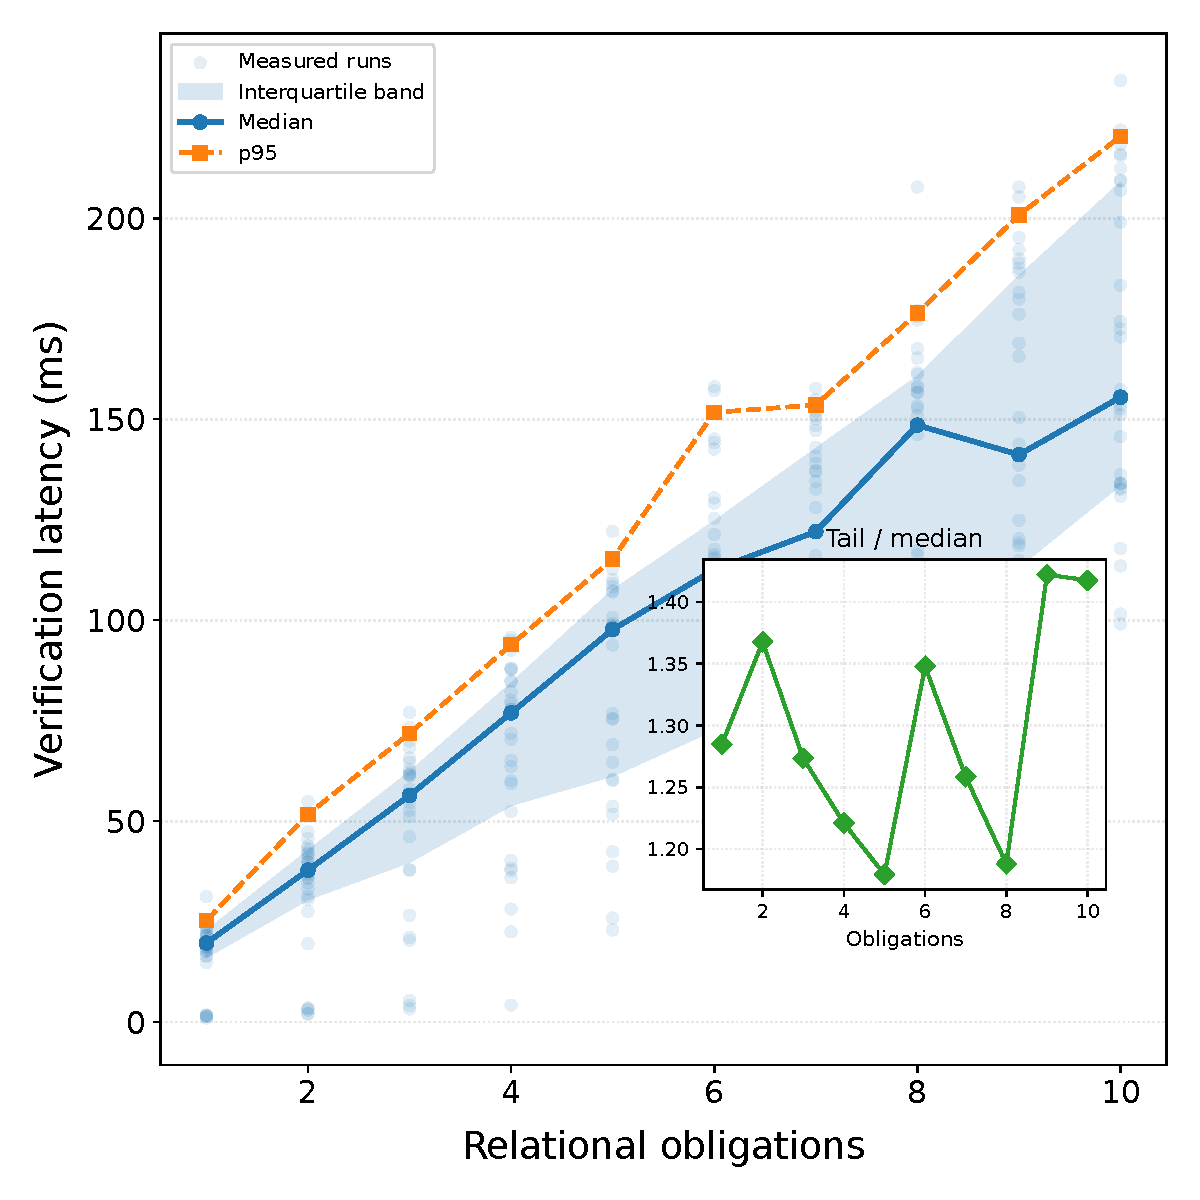
\includegraphics[width=\linewidth]{dataset/results/figures/figure_scalability_obligations.pdf}\\[-1mm]
\scriptsize (a) Relational obligations
\end{minipage}\hfill
\begin{minipage}[t]{0.485\textwidth}
\centering
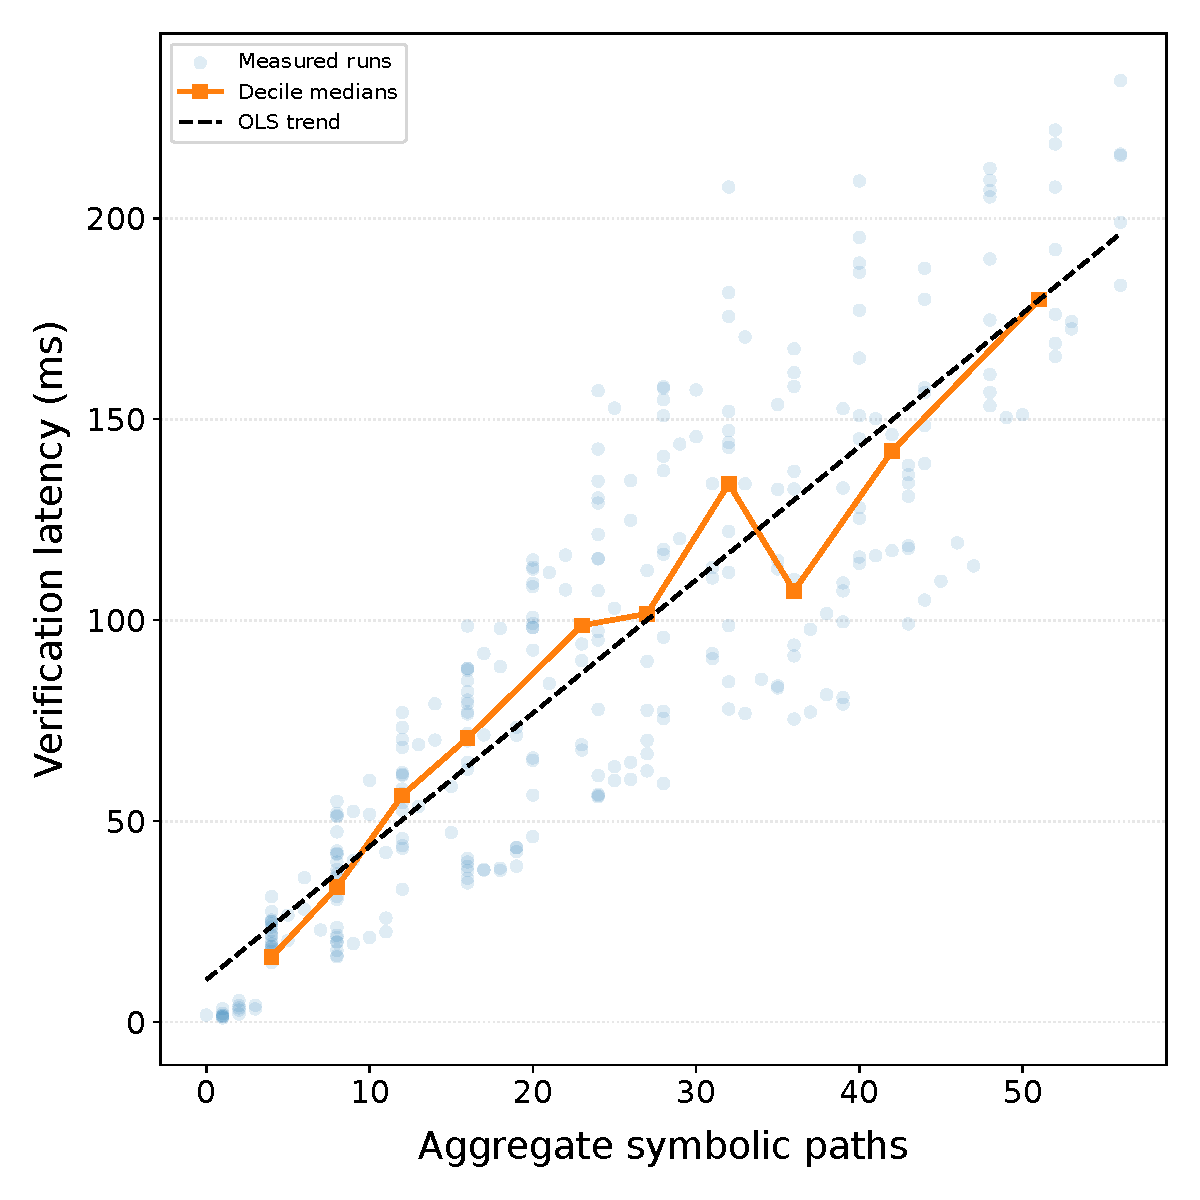
\includegraphics[width=\linewidth]{dataset/results/figures/figure_scalability_paths.pdf}\\[-1mm]
\scriptsize (b) Symbolic-path mass
\end{minipage}
\caption{Scalability under controlled relational batches.  Panel (a) retains all runs, the interquartile band, median, p95, and an inset tail ratio. Panel (b) overlays decile medians and the OLS trend on all path-count observations.}
\label{fig:scalability}
\end{figure*}

Figure~\ref{fig:scalability} shows median latency increasing from 19.63\,ms for one obligation to 155.46\,ms for ten.  Ordinary least squares gives 16.45\,ms per added obligation with \(R^2=0.724\), while symbolic-path mass explains slightly more variance with \(R^2=0.767\).  For observation \(i\), the centered models are
\begin{equation}
 T_i-\bar T=\beta_o(o_i-\bar o)+\varepsilon_i^{(o)},\qquad
 T_i-\bar T=\beta_p(p_i-\bar p)+\varepsilon_i^{(p)},
\label{eq:scaling-model}
\end{equation}
where \(o_i\) and \(p_i\) denote obligations and aggregate symbolic paths. The reported coefficients minimize \(\sum_i(\varepsilon_i^{(\cdot)})^2\), while the figures separately retain nonparametric conditional medians.  Their agreement supports a monotone interpretation over the controlled range, not an asymptotic solver guarantee.

\section{Discussion}
\label{sec:discussion}

The experiment exposes two distinct conservatism choices.  Layout name matching rejects a physically safe internal rename, producing seven false alarms.  Removing names entirely is not sufficient, because two declarations can share width and position but differ in interpretation.  A robust successor should infer correspondence from qualified declaration identity, access patterns, and user-confirmable matches.

Behavioral under-approximation has the opposite failure mode.  The current summary grammar does not lower conditional effects, revert payload bytes, or Keccak expressions into Eq.~\eqref{eq:product}.  Unsupported cryptographic expressions become \(\Unknown\), but the conditional cases demonstrate that frontend incompleteness can still yield a false proof.  Closing this gap requires a control-flow-sensitive SSA frontend whose soundness is related to Solidity/EVM semantics, not additional ad hoc patterns.

The artifact separates three evidence levels: a compiler-grounded structural diagnosis, an SMT witness checked by an independent interpreter, and an actual EVM replay.  This separation is useful operationally.  A developer can inspect the exact byte footprint for a layout issue or replay a behavioral witness, while an \(\Unknown\) remains an explicit review obligation.

\section{Threats to Validity}
\label{sec:threats}

\textbf{Construct validity.} Mutation labels represent controlled hazards, not incident frequency. The deterministic fuzzer is a bounded baseline and is not Forge's built-in fuzzer.  ``Safe'' from the relational stage means unsatisfiable only in the implemented model and domain.

\textbf{Internal validity.} The generator, detector, and evaluator share a repository, but ground-truth validation does not call the proposed detector.  Compiler success, mutation realization, artifact completeness, and duplicate hashes are checked separately.  Anvil replay adds independent bytecode-level evidence for counterexamples, although it does not validate proofs.

\textbf{External validity.} The corpus contains 20 generated originals and no production upgrade history; Table~\ref{tab:related} therefore marks real-corpus support as absent.  Results may not generalize to inline assembly frameworks, diamonds, custom namespaced storage, delegate-call chains, or arbitrary cross-contract behavior.

\textbf{Conclusion validity.} Repeated timings share one workstation and are not independent hardware replications.  We retain raw rows, report medians/IQR/p95, and avoid exact boundary percentages.  The scaling regression is descriptive over batches one through ten.

\section{Conclusion}
\label{sec:conclusion}

\tool demonstrates that upgrade checking benefits from treating physical state compatibility and behavioral preservation as one selective relational problem.  The artifact is fast on its supported subset and produces EVM-replayable witnesses, but its value is also in the failures it exposes: name-based false alarms, computed assembly unknowns, and conditional/revert semantics beyond the current frontend.  The next step is a control-flow-sensitive, semantics-linked encoder evaluated on independently collected production histories; the present controlled corpus and raw pipeline provide a reproducible baseline for that work.

\begin{credits}
\subsubsection{\ackname}
No external funding was declared for this study.

\subsubsection{\discintname}
The authors have no competing interests to declare that are relevant to the content of this article.
\end{credits}

\bibliographystyle{splncs04}
\bibliography{ref}

\end{document}
